% !TEX TS-program = xelatex
% !TeX spellcheck = en_GB
% !TeX root = ../My_thesis.tex

\chapter{Summary of the Methodology}\label{chap:method}
\red
\section{Overview}
	In this chapter, an overview on modelling strategies in micro-mechanics is presented, and the conceptual view towards developing computer programs is briefly reviewed. Programming paradigms have been often overlooked, and thus the approach to programming is not quite `structured'. After elaboration on the philosophy of common programming approaches, the capabilities of the Marc/Mentat semi-open software package is reviewed. Finally, the progress of code development for the in-house program of the current thesis is summarised. This chapter is certainly not a comprehensive and detailed explanation of all the programming effort but at least, it could shed some light over the reader's path so the coherence of the whole work becomes more evident.

\section{Modelling Strategies in Micro-Mechanics}
	\paragraph{Terminology} Since `macro' and `micro' terms are merely used to indicate the difference in the size of their scales (rather than pointing to an explicit length domain), the more general `coarse' and `fine' terms would be better alternatives in that sense, respectively. Often the intermediate scales between the mentioned ones are called the `meso-scales'~\autocite{Bohm.2020}. Transferring information from a macro to micro scales is called \textit{downscaling} or \textit{localisation} whereas any movement in the opposite direction is called \textit{upscaling} or \textit{homogenisation}. 

	\paragraph{Principle of separation of scales} Depending on the way length scales are dealt with, concurrent or hierarchical methods could be used. In the former, both macro and micro scales refer to the same length scale whereas in the latter, the scales are separated. Thus, \textit{the principle of separation of scales}~\autocite{Geers.2010} is adopted. Namely, the micro-scale model is a representative volume element of the macro-scale one, which means it is small enough to represent the microstructure and at the same time large enough so the continuum mechanical equations remain valid. Mathematically, this assumption is denoted as
	\begin{equation}
		\ell_\text{heterogeneities} \ll \ell_\text{fine} \ll \ell_\text{coarse},
	\end{equation}
	where $\ell$ is a characteristic length. This relation emphasises that in order to deal with the micro scale as a (classic or generalised) continuum, the length scale must be taken large enough compared to its heterogeneous components. The assumption becomes invalid when the macro and micro scales are of the same length or a localisation happens in the macro scale, e.g., due to initiation of cracks~\autocite{Spahn.2015}. In such cases, a single RVE ceases to represent the macro scale and the principle of separation collapses.
	
	\paragraph{Multi-scale modelling} A localisation/homogenisation setup is referred to as \textit{multi-scale modelling}, which is carried out in coupled and uncoupled modes. In the uncoupled version, only upscaling is done, i.e., the effective properties are computed (or even pre-computed) from the RVE and used as the properties of the macro continuum. The exchange of information is one-way: from micro to macro. On the contrary, in the coupled version, both upscaling and downscaling take place. Namely, in the framework of finite element method (FEM), for every integration point of the macro structure, an RVE is assigned to provide the macro response at the point. A two-way exchange of information is required in this case. The most famous example of this method is the FE$^2$ approach~\autocite{Feyel.1999}, which was later extended to a coupling between micro-scale classic continua and macro-scale non-Cauchy continua~\autocite{Feyel.2003}. From another perspective towards generalised continua, the first- and second-order homogenisation/localisation schemes are mentionable. In the first-order scheme, only the deformation gradient is the carrier of the kinematic deformation in downscaling while its gradient is deemed negligible~\autocite{Kouznetsova.2002}. In contrast, the second-order scheme requires the first gradient of the deformation gradient to be transferred. In any case, most of the multi-scale schemes require high-performance computation resources, which is a major draw-back. Overall, complexity of the multi-scale methods, specially the coupled version, in both implementation and computation makes them a less attractive alternative in application.
		
	\paragraph{Single-scale modelling} Establishing the one-way localisation/homogenisation relations depends on how the interaction of the constituents is considered; two main categories exist~\autocite{Bohm.2020}:
	\begin{enumerate}
		\item \textit{Collective description} where the heterogeneities are not considered explicitly but in an average sense. Most of the methods under this category follow the \textit{mean-field approach} (MFA), and could be considered as special cases of \textit{Hashin-Shtrikman estimates} by changing the reference material~\autocite{Bohm.2004}; more specifically, they are divided into the following sub-categories\,\footnote{The \textit{effective self-consistent scheme} is also available in the literature, see~\autocite{Zheng.2001}.}:
		\begin{itemize}
			\item \textit{Effective field approach} (Mori-Tanaka approach~\autocite{Mori.1973}) where the stress/strain in the inhomogeneity is related to the average values of stress/strain of the matrix. In this model, the inhomogeneity is incorporated into the matrix, i.e., the matrix is the reference material.
			\item \textit{Effective medium approach} (family of self-consistent schemes~\autocite{Hill.1965}) where the inhomogeneity is incorporated into an effective material. The requirement of the model is that the perturbation caused by introducing the inhomogeneity in the effective material must vanish, i.e., the effective material is the reference material.
		\end{itemize}
		Often, the interaction of the constituents is considered overall (statistically) or just simply ignored, e.g., in Eshelby dilute approximations~\autocite{Eshelby.1957}. 		Additionally, \textit{bounding methods} are also categorised under MFA, e.g., the strength-of-material approaches known as Voigt~\autocite{Voigt.1889} and Reuss~\autocite{Reuss.1929} bounds or altogether in tensorial form as Hill bounds~\autocite{Hill.1951,Hill.1963}, Hashin-Shtrikman-type bounds~\autocite{Hashin.1962,Hashin.1963}, or their extended version~\autocite{Walpole.1966,Walpole.1969}, etc. where usually variational principles are used to estimate them~\autocite{Mura.1992,Hu.1984}.
		\item \textit{Discrete description} where discrete heterogeneities are modelled with the aim of fully capturing the constituent interactions---and thus called the \textit{full-field approaches} (FFA). Depending on the available symmetry of the microstructure, different methods could be used. For instance, unit cell methods are made available by taking advantage of a periodic microstructure (periodic RVs). Otherwise, sampling methods (or windowing approach), embedding approach or for the extreme case of non-period microstructure, modelling discrete heterogeneities could be used~\autocite{Bohm.2020}. The solution of the RVs can be obtained computationally by the finite element method (FEM), boundary element method, fast Fourier transformations (FFT), transformation field analysis~\autocite{Dvorak.1992,Dvorak.1992b} etc.
	\end{enumerate}
	For a more formal and comprehensive description of the aforementioned schemes see~\autocite{Mura.1987,NematNasser.1993}.

	The accuracy-cost trade-off is quite obvious in each category; calculations of the MFAs and bounds are inexpensive whereas the FFAs could be time consuming.\,\footnote{Except for the FFT method, which is quite efficient but could not easily be used in parallel computing~\autocite{Matous.2017}.} In contrast, the interaction of the constituents is captured with better accuracy using FFAs among which FE analysis is frequently used. Attempts were made to obtain better MFAs by refining the homogenisation approach, e.g., see the two-step homogenisation scheme~\autocite{Pierard.2004,Doghri.2006}. The application of several MFAs and FFAs are available in~\autocite{Muller.2015}.
	
	Considering the drawbacks of each method, combining both methods seems to produce better hybrids. For instance, in the context of FEA, MFA could be implemented at the level of elements (see Chapter~\ref{chap:p7}) and the solution is obtained for any arbitrary geometry.

% --------------------------------------------------------------------------------------------------
\section{Modelling Damage}
	\paragraph{Direct modelling of damage} Softening behaviour is the characteristic of damage progression. For an isotropic damage measure, a scalar value is adequate while quantification of anisotropic damage requires a tensor field. To consider softening, three basic types of damage models are recognised~\autocite{Bazant.1998}:
		\begin{enumerate}
			\item elastic softening with stiffness degradation (pure damage): continuum damage models that incorporate post-yield elastic modulus reduction without any plastic deformations,
			\item yield limit degradation with plasticity (pure strength degradation): that incorporates post-yield yield stress reduction while elastic modulus remains constant, and
			\item the mixed theory that combines both of the aforementioned effects.
		\end{enumerate}
		
	\paragraph{Consequences of softening behaviour} Introducing a softening effect in the stress-strain response of the material is carried out by incorporating a damage parameter in the model. However, the softening behaviour often causes numerical issues since it is inherently an ill-posed problem~\parencite{Jirasek.2007b}---it does not converge to a rational value upon mesh refinement, and at the same time produces a finite change in the solution due to an infinitesimal perturbation of the input~\autocite{Jirasek.2002}. Point-wise loss of stiffness causes highly localised and infinitely large strains, i.e., the smaller the element size, the more localised the strain becomes and the larger its magnitude would be. Such strain fields require regularisation by enforcing some conditions---the so-called \textit{localisation limiters}.

	\paragraph{Inelasticity prior to the peak} The softening effect can be considered post-peak or pre-peak in the stress-strain curve~\autocite{Bazant.1998}. Namely, the pre-peak nonlinearity (if any) can be modelled by introducing an early stiffness/strength degradation in the material.	

	\paragraph{Indirect modelling of damage} Provided that the microstructure of the material is statistically well-characterised (i.e., properties and distribution of the heterogeneities), there is no need for direct measurement of the damage parameters in macro-scale. In such cases, the evolution of damage, at least for a monotonic loading, can be modelled \textit{indirectly} via modifying the heterogeneities~\autocite{Bazant.1998}. The extreme case of this modification is removing the meso-scale material completely. 
	
	\paragraph{Element elimination technique} Deactivating the elements during analysis mimics the loss of stiffness/strength in the material. \textit{Element elimination technique} (EET) was used to predict crack propagation in a homogeneous material~\parencite{Wulf.1994}. The \textit{multi-phase element method}~\parencite{Steinkopff.1995} was used when one type of element represents two different phases. By adopting a similar approach, it is suggested to model damage for embedded elements in a composite material.
	
	\paragraph{Deactivation of the elements in composites} Adopting an element deactivation process for the matrix, similar to that of the fibres, seems to be too simplistic and harsh to the solver. However, it follows the weakest link idea that failure is initiated from the weakest point~\parencite{Jirasek.2007}.	Nevertheless, sudden removal of the matrix elements might cause convergence problems due to the mentioned ill-posedness, and thus a smoothing process might be required, e.g., displacement averaging~\parencite{Jirasek.2005}. This problem is not severe for the case of embedded fibre elements because failure of a fibre element might generate two smaller fibres---each one is deemed to be stronger than the parent one in the proposed strength-updating model, see Chapter~\ref{chap:p6}. Thus, the sudden loss of strength and premature failure of the specimen does not follow. 
 


\section{Programming Life Cycle}
	Computer programming is usually considered as merely writing a piece of code, but in fact it consists of several processes in a closed circuit, see Fig.~\ref{figure:programdevelopment}. More precisely, the life cycle of developing a program consists of the following stages:
	\begin{itemize}
	\item understanding the problem, 
	\item planning the logic, 
	\item writing the code, 
	\item compiling and debugging, and
	\item documenting, maintenance, and updating.
	\end{itemize}

\begin{figure}[!t]
	\centering
	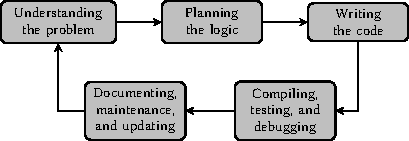
\includegraphics[scale=1.25]{life_cycle.pdf}
	\caption{Iterative steps of program development}
	\label{figure:programdevelopment}
\end{figure}%	
	
	Understanding the problem involves identifying the tasks, which should operate on the inputs to produce the desired outputs. There is a certain aim for the program to achieve and this is done by processing the inputs. The goal is materialised when the targeted output is generated. At the end of this stage, the objective, input(s), and output(s) of the whole program are clearly defined. In addition, the existing limitations may be identified.

	In the logic planning stage, the algorithm of the program is developed, which determines the mechanism of each task. As the goal is already known from the previous step, now it is the time to go into the details of the design. The final goal is divided to several tasks, and every step of each task is carefully determined---following the principle of `divide and conquer'. At the end of this stage, it will be known in detail that how each task is going to be done, i.e., the algorithm is generated. The description of the algorithm can be in the form of flowcharts and/or pseudo-codes.
	
	The developed algorithm is implemented by obeying the syntax of a specific programming language. Namely, the programmer must obey the syntactic rules of the selected programming language; this is commonly called `programming'. It is analogous to obeying the grammar in writing a piece of literature. At this stage, all the tasks are translated from a common language to several lines of programming code.

	The compiled code can be tested by feeding various inputs and checking the outputs for correctness.\,\footnote{Compiling is translating the lines of code from a low- or high-level programming language to the lowest possible level, i.e., the machine code. Examples are \f and C/C++. It is called \textit{interpretation} if no intermediate object files are generated and the syntax checking is partially done upon execution, e.g., \py.} In this process both the syntactic and possible semantic errors are revealed and debugged. The errors pertaining to the syntax and those resulted from an irrational logic should be re-addressed in the code writing and logic planning stages, respectively.
	
	Documenting not only helps maintaining the code but also reassures that the development life cycle can continue. Several documents are generated to facilitate this process. For instance, the \textit{programmer documentation} helps the programming team to maintain the current code while the \textit{user documentation} provides users with useful information on utilizing the program. On the other hand, the bug reports or demands from the users push the cycle forward for further updates.
	
	Some of the mentioned steps may be done concurrently, and thus one cannot draw definite borders between them. Another possibility is the limitations in one step, which may require going back several steps to amend the source. For instance, there may be a case in which writing the code for the planned task is not possible in a particular programming language, and therefore the logic should be modified. Or sometimes even the issue is traced back to a defective design. The result is having mini cycles within the grand cycle of programming development. No matter how each step is performed, the introduced cycle is effective in producing programming codes on a solid foundation. Careful time investment in each step will save effort in the subsequent ones and increases the longevity of the program. 

\section{Imperative \& Declarative Programming Paradigms}
	Among the mentioned steps of program development, `planning the logic' lays the structure of the program; yet, it is usually taken for granted. The logic is highly affected by how the programmer thinks. The extent of freedom in his/her thinking is limited by the provided constructs of the programming language---which is dictated by the supported programming paradigms of that language. Thus, the supported paradigms of the programming language limits the free thinking of the program developer. An overview of major programming paradigms will be introduced in this section.

	A \textit{programming paradigm} defines the perspective of the programming language towards tackling a programming task; it is the overall philosophy of the programming language. For instance, it tells the programmer to see the problem as a few interacting objects or merely consecutive lines of commands. In either way, the problem will be addressed, but different paths will be taken. Programming paradigm dictates this path.
	
	A paradigm to its programming code is like a mathematical model to its solution. Different paradigms will generate different programming codes as different models result in possibly different mathematical solutions. Paradigms provide answers to a specific problem by means of different approaches. Similarly, different mathematical models can be used to capture the behaviour of a physical phenomenon, which finally result to possibly different answers. 
	
	Every paradigm is based upon certain concepts, and thus it alters how the programmer thinks, designs, and writes the code. Therefore, the selected paradigm mostly affects the steps of planning the logic, and consequently writing the code during the development life cycle.
			
	There are very few programming languages which purely target a certain paradigm. As a matter of fact, some programming languages are intended to support several paradigms---called \textit{multi-paradigm languages}. A good example is Leda which supports imperative, object-oriented, and declarative (both functional and logical) altogether. The basic idea behind multi-paradigm languages is that programmer can adopt and mix the required constructs from different paradigms according to the nature of the problem in-hand since there is no single perfect paradigm for every possible purpose~\autocite{Budd.1995}.
	
	The second reason for having a small number of pure paradigm languages is the fact that most paradigms have many overlapping features with other ones which makes it almost impossible to create a pure programming language. Nevertheless, Haskell and SequenceL as pure functional languages and Smalltalk as a pure object-oriented language are mentionable.
	
	Although a multi-paradigm programming language may provide facilities for several programming paradigms but usually it is well-suited, or at least famous, for a specific one. For example, \py{} provides the required facilities for object-oriented programming (OOP) along with many imperative structures. However, it is mostly known as an OOP language for its dominant capabilities in handling objects.
		
	Since there are many common concepts between distinct paradigms, categorising programming paradigms becomes rather complex, for a taxonomy see \autocite{vanRoy.2009}. However, a brief description of the major paradigms will help a programmer to understand which parts of a certain programming language he/she is touching. 

	\paragraph{Imperative programming} In an \textit{imperative} paradigm, the program consists of several consecutive `statements'\,\footnote{Note that in the context of the low-level imperative programming languages the term \textit{statement} is used for what is being executed whereas in a high-level one, the term \textit{command} is preferred~\autocite{Normark.2003}.}. Namely, the paradigm enforces a step-by-step execution of a procedure to achieve a goal. 
	
	The important consequence of executing several statements is changing the \textit{machine state} or \textit{program state}. The state of a program at each moment is defined by the state of the memory at that moment, i.e., the stored data and the reserved block of data in the memory. Therefore, the state of a program changes by changing the content of the memory as well as reserving or releasing blocks of it. For instance, state changes by creating or removing a variable; modifying the value of a variable; or even assigning a pointer to a memory location.

	Most of the conventional programming languages, such as C/C++, incorporate the imperative paradigm since it is the closest form to the machine code. Therefore, efficiency usually accompanies lower-level programming languages. Nevertheless, handling large pieces of code in this way is very demanding. Therefore, the imperative approach was refined in many ways to handle larger pieces of code more easily. It branched to other programming paradigms such as the \textit{structured programming}.
	
	Introducing structured programming~\autocite{Dahl.1972} dates back to late 1950s, which later resulted in the \textit{structured program theorem} or \textit{B\"ohm-Jacopini Theorem}~\autocite{Bohm.1966}. The essence of the theorem is that no matter how complicated the task is, a structured program can deal with it using an orderly combination of the following basic structures:
	\begin{itemize}
	\item a \textit{sequence} which is a series of processes,
	\item a \textit{decision} which tests a logical value, and
	\item a \textit{loop} which is used for repeating structures.
	\end{itemize}
	The `combination' of these structures cane be done in two ways: either they can be placed one after another to make up a block---called \textit{stacking}---or placed within each other---called \textit{nesting}.
	
	The most prominent and disputed characteristic of a structured program is the rule of `single-entry single-exit point'. Namely, the execution of the code block must start only at one point and end only at one point, i.e., no jumps are allowed between various points of the code. Complying with this rule is only possible by prohibiting the use of any \code{GOTO} statements. Thus, structured programs are often called \code{GOTO}-less programs.

	The characteristics of a structured program can be summarised into the following points:
	\begin{itemize}
	\item A structured program is a nested and/or stacked combination of sequences, decisions, and loops.
	\item One-entry one-exit point rule applies to the flow of the program---no jumping is allowed.
	\item In a loop structure, the control of the program must return to the decision structure after finishing the loop.
	\item The decision structure divides the flow of the program to two paths. These paths must join together later but they cannot return to the decision structure.
	\end{itemize}
	Any unstructured program can be put into a structured form by using some additional statements, auxiliary variables, or recursive procedure calling, see~\autocite{Farrell.2015} for some examples.
	
	Several other famous paradigms have been derived from the structured paradigm such as \textit{procedural}, \textit{modular}, and \textit{object-oriented} paradigms. Each of these paradigms stayed faithful to their ancestor while adding new concepts to its philosophy.
	
	A \textit{procedural} programming approach breaks down the whole process into several procedures. Using the `divide and conquer' rule, a complex task is broken down to several simple manageable procedures. Each procedure is usually a small piece of code which is wrapped in a programming structure. It is called by different names in different programming languages such as method, subroutine, function, and procedure. While all of the aforementioned terms incorporate procedures, minute differences exist between them. 
	
	In the procedural approach, the main code makes a procedure call and the intended procedure is executed. The called procedure might also call other procedures. However, this network of calls is not necessarily independent of each other. The dependency is introduced when variables of the caller are used in the called procedure by any mechanisms other the arguments and returned values. Being dependent on the state of the caller makes tracking changes and modifying the procedures cumbersome. By increasing the independence of procedures and decreasing their side effects, the code becomes more `modular'.
	
	The \textit{modular paradigm} is an extension to the structured procedural paradigm. Both of them date back to 1960s but modular programming became popular in 1980s along with introducing \textit{units} in Pascal. In early 1980s, C++ programming language was born by combining the features of C and the objects of a simulation programming language named Simula~67~\autocite{Deitel.2006}. It took some time until 1990s for the object oriented programming to gain attention by the help of C++ programming language while refusing any support for modularity.\,\footnote{Interestingly, \py{} has incorporated both modular and object-oriented paradigms since its early days of development in 1990s.}
	
	The idea behind the modular paradigm is to incorporate interchangeable independent parts of code. Namely, the code is divided to independent procedures which can be easily rewritten or replaced without affecting the main code. Therefore, a modular design increases the re-usability of the code compared to when only a large piece of code is developed. The created modules can be easily used in other projects often without any changes. Furthermore, it facilitates group work since each team member can design the required module without really considering the interactions the module with other parts.
	
	\paragraph{Declarative programming} The \textit{declarative paradigm} is the opposite point of the imperative paradigm since it only defines what is the required result not the implementation steps for obtaining it. Database query languages, such as structured query language (SQL), use the declarative approach. For instance, you only ask for the name of all your customers by a single line of code and you get access to the information without going through the details of managing a database. Two distinctive programming paradigms, which have acquired the declarative approach are \textit{logical programming} and \textit{functional programming}.
	
	Every algorithm is decomposed eloquently into two constituents~\autocite{Kowalski.1979}:
	\begin{equation*}
	\text{Algorithm}=\text{Logic}+\text{Control}.
	\end{equation*}
	The logical paradigm focuses merely on the logic part of the algorithm while ignoring the details of the control structures. Again, here the focus is on what should be done (the logic component) and not on how it should be done (the control component).

	%TODO this paragraph requires refinement
	Obviously in an imperative approach, the programmer is responsible for both the logic and control components. Thus, improving the efficiency of the code is done by improving either or both of the components. However, it is argued that the logical approach makes the improvements easier since it separates these two components and focuses only on the logic part while using the facilities of `intelligent theorem-proving systems'~\autocite{Kowalski.1979}.
		
	The \textit{functional paradigm} tends to mimic mathematical functions and remove the need of using variables by a composition of functions. Programming functions can act as mathematical functions if they can accept functions as arguments, return results as functions rather than variables, and always give the same result for the same arguments at all times---it is the quality of being \textit{atemporal} just like a mathematical function. Therefore, instead of engaging variables and advancing through different states, as in an imperative paradigm, nested functions are evaluated. Thus, the concept of `state' is not applicable since values are not stored and modified as variables~\autocite{Budd.1995}. Namely, values are fixed, and thus any computation will not modify them but it creates a new value. A careful design using these facilities can result in an easy-to-understand succinct and efficient program~\autocite{Lott.2015} while minimizing the \textit{side effects} of the code, i.e., the state changes.

	A summary of the major paradigms is listed in Table~\ref{table:paradigms}. One should pay attention to both \py\ and \f\ since these are the two most used programming languages in the context of finite element modelling. Relating their supporting paradigms, it is notable how most of the imperative family of paradigms is covered by these two programming languages.
		
\begin{table}[!h]
\centering
\caption{Selected programming languages and their supporting paradigms}\label{table:paradigms}\small
\begin{tabular}{p{0.16\textwidth}@{}p{0.35\textwidth}p{0.425\textwidth}}
	\toprule
	\bfs{Paradigm}     & \bfs{Intuitive description}              & \bfs{Supporting languages}            \\ \toprule
	Imperative                    & Do this, then that                 & Fortran, Python, ALGOL, Basic, Pascal, and C/C++ \\
	Structured                    & One-entry one-exit (avoid jumps)   & Fortran, Python, the C family, BASIC, and Pascal     \\
	Procedural                    & Break down to procedures           & Fortran, Python, ALGOL, BASIC, Pascal, and C     \\
	Modular                       & Break down to independent modules  & Fortran, Python, ALGOL, Pascal, and C\#          \\
	Object-oriented               & Everything is an object            & Python, Smalltalk, C++, C\#, and Java               \\ \midrule
	Declarative                   & Explain what is to be done not how & SQL, and Wolfram                             \\  
	Functional                    & Avoid variables, use functions     & Haskell, SequenceL, Lisp, Python, and the C family \\
  Logical                       & Only define the logic                & Prolog                           \\  \bottomrule
\end{tabular}

\end{table}

As a by-product of the current thesis, about 50 customised subroutines in \f\ has been developed and published in~\autocite{Javanbakht.2017}. Adopting the concept of modularity, all these subroutines are reusable. More importantly, they have been used in the conducted finite element analyses of the current study. Moreover, in order to take advantage of most of the imperative paradigms, both \f\ and \py\ languages were used in developing the code. More specifically, the OOP was engaged by means of \py. In the following section, the particular role of each of these components is discussed in the context of the \mm\ commercial package.
	 
\section{Modern Finite Element Programming}
	Conventional finite element (FE) problems are easily handled by commercial software packages. Other more complicated tasks require writing in-house programs that have a long development timeline. Moreover, programming a solver (specially a parallel one) for the recurring simultaneous system of equations is non-trivial. Most of the available commercial FE packages adopt a black-box approach and do not allow the user to customise the critical parts. Obviously, the open-source FE packages are more compliant in this sense; nevertheless, they lack the vigorous support and updates of their commercial counterparts. 
	
	Currently, the ABAQUS and MSC \mm{} packages allow partial modification of their critical code; since the latter offers more flexibility in terms of number of subroutines, it is selected for the current study. The result was saving time by avoiding any code development for the trivial parts of solution procedure and focus more on the critical parts, i.e., the model development, constitutive behaviour, and implementing new finite elements among others. In the sequel the features of this commercial package is reviewed more closely.
	
The \mm{} commercial finite element software is a multi-physic simulation package, which provides a good collection of \f{} subroutines. These subroutines allow the user to customize the program for carrying out non-standard finite element tasks, see for instance~\autocite{Javanbakht.2017}. Furthermore, the capability of scripting releases the user from laborious and repetitive tasks of preprocessing such as creating geometries, nodes, elements, meshing, applying boundary conditions, assigning materials, and creating sets; and post-processing such as result collection, manipulation, and conditional job re-submissions.

The pre-, and post-processor of the \mm{} package is called \M{}, which is merely a graphical user interface (GUI). However in the background, the solution of the finite element analysis is carried out by \m{}. This interaction involves several input, output, and auxiliary files, see Fig.~\ref{figure:marc_mentat}. \M{} carries out all the preprocessing tasks which results in an input file (\code{.dat}). Note that while working with the GUI a log file (\code{mentat.log}) and a procedure file (\code{mentat.proc}) is created. This procedure file is important because it records all the activities of the user since the start of program which can be used for the following purposes:
\begin{itemize}
\item as a backup for the current model that can be used to repeat all the user actions, or
\item as as starting point for creating customized procedure files by the beginner users.
\end{itemize}

	\begin{figure}[!h]
	\centering
	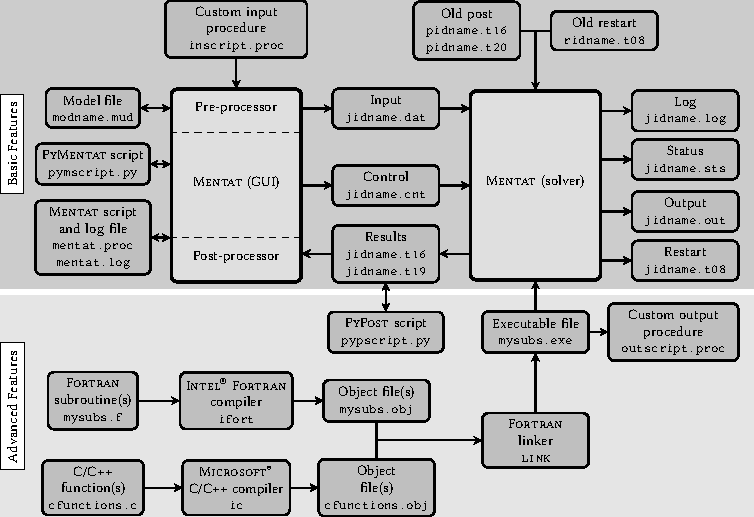
\includegraphics[width=\textwidth]{marc_mentat.pdf}
	\caption{\pym{} and \pyp{} interaction with other components of \mm{}}\label{figure:marc_mentat}
	\end{figure}

The created finite element model can be saved as a binary file in a model file (\code{.mud}) or it can be written to a text file called an input file (\code{.dat}). This file is submitted as a job to the solver, i.e., \m{}, along with any possible \f{} subroutines (\code{.f}). %TODO see if the free format is possible to run now in the new version
During running the job a log file (\code{.log}), a status file (\code{.sts}), an output file (\code{.out}) and more importantly a result file (\code{.t16} or \code{.t19}) is produced among others. The result of the analysis can then be visualized, collected and modified using \M{}. All these features are `basic' and are used several times in common FE analyses.
 
The aforementioned process is quite straightforward when dealing with simple models or when dealing with a handful of models. Analysing such cases become exhausting when several job resubmissions are inevitable; and even more cumbersome when there is a condition which determines if the submission is required or not. In such cases, moving to the `Advanced' features is inevitable. Two remedies are provided by the package to deal with such difficulties: procedure files and \py{} scripts. The latter case is more general where looping and conditional statements are allowed where the former is readily used for parametric model generation.


\section{Development of the Methodology}
	One other point of using the advanced features of Marc/Mentat is that without the need of going into the details of solvers and GUIs, one could take advantage of the flexibility provided by the subroutines, i.e., to create new constitutive laws, and new finite elements, which are frequently use in the state-of-the-art research. In this section, a brief overview of the progression that occurs in the following chapters is presented; the aim is to clarify what features have been developed for the in-house program in the course of research. By no means this would a thorough description of the programming code as it is not practical to provide a line-by-line description. The development of the programming code can be viewed from three perspectives: types of analyses, capabilities, and the used programming paradigms; see Table~\ref{table:inhouse}.


\begin{table}[!h]
\caption{Summary of the developed features in the in-house program (non-chronological)}\label{table:inhouse}\small\centering
\begin{tabular}{l*{7}{P{0.05\textwidth}}}
\toprule
\multirow{2}{*}{\bfs{Feature}} &\multicolumn{7}{c}{\bfs{Chapter}}\\\cmidrule(l{0.2cm}r{0.2cm}){2-8}
                               &\bfs{4}&\bfs{5}&\bfs{6}&\bfs{7}&\bfs{8}&\bfs{9}&\bfs{10}\\
\toprule
\multicolumn{8}{c}{\small Analysis type}\\
\midrule
2D RVE                                   &\cmark&\cmark&\cmark&\cmark&\cmark&\cmark&\cmark\\
3D RVE                                   &\cmark&\cmark&\cmark&\cmark&\cmark&\cmark&\cmark\\
Transverse RVE                           &\xmark&\xmark&\xmark&\cmark&\xmark&\xmark&\xmark\\
Synthetic fibres                         &\cmark&\cmark&\xmark&\cmark&\cmark&\xmark&\xmark\\
Natural fibres                           &\xmark&\xmark&\cmark&\xmark&\xmark&\cmark&\cmark\\
Discontinuous fibres                     &\cmark&\xmark&\xmark&\cmark&\cmark&\cmark&\cmark\\
Continuous fibres                        &\xmark&\cmark&\cmark&\xmark&\xmark&\cmark&\cmark\\
Thermal analysis                         &\cmark&\cmark&\cmark&\cmark&\cmark&\xmark&\xmark\\
Mechanical analysis                      &\xmark&\xmark&\xmark&\xmark&\xmark&\cmark&\cmark\\
Clustering analysis                      &\xmark&\xmark&\xmark&\cmark&\cmark&\xmark&\xmark\\
Spectral analysis                        &\xmark&\xmark&\xmark&\cmark&\cmark&\cmark&\cmark\\
Sensitivity analysis                     &\cmark&\cmark&\cmark&\cmark&\cmark&\cmark&\cmark\\
\midrule
\multicolumn{8}{c}{\small Capabilities of the program}\\
\midrule
Randomly-oriented fibres                 &\cmark&\cmark&\cmark&\cmark&\cmark&\cmark&\cmark\\
Variable fibre volume fraction           &\cmark&\cmark&\cmark&\cmark&\cmark&\cmark&\cmark\\
Arbitrary fibre length distribution      &\xmark&\cmark&\cmark&\cmark&\cmark&\cmark&\cmark\\
Arbitrary fibre orientation distribution &\cmark&\cmark&\cmark&\cmark&\cmark&\cmark&\cmark\\
Arbitrary fibre strength distribution    &\xmark&\xmark&\xmark&\xmark&\xmark&\cmark&\cmark\\
Arbitrary fibre CSA distribution         &\xmark&\xmark&\xmark&\xmark&\xmark&\cmark&\cmark\\
Matrix mesh density control              &\cmark&\cmark&\cmark&\cmark&\cmark&\cmark&\cmark\\
Fibre mesh density control               &\xmark&\xmark&\xmark&\xmark&\xmark&\cmark&\cmark\\
Embedded elements technique              &\cmark&\cmark&\xmark&\cmark&\cmark&\cmark&\cmark\\
Aligned fibre generation                 &\xmark&\cmark&\cmark&\cmark&\cmark&\cmark&\cmark\\
Variable fibre length                    &\xmark&\cmark&\cmark&\cmark&\cmark&\cmark&\cmark\\
Fibre volume fraction correction         &\xmark&\cmark&\cmark&\cmark&\cmark&\cmark&\cmark\\
RVE sub-partition generation             &\xmark&\xmark&\xmark&\cmark&\cmark&\xmark&\cmark\\
Element elimination technique            &\xmark&\xmark&\xmark&\xmark&\xmark&\cmark&\cmark\\
Fibre strength updating                  &\xmark&\xmark&\xmark&\xmark&\xmark&\cmark&\xmark\\
Fibre efficiency considerations          &\xmark&\xmark&\xmark&\xmark&\xmark&\cmark&\cmark\\
Independent RVE import/export            &\xmark&\xmark&\xmark&\xmark&\xmark&\xmark&\cmark\\
Localised homogenisation formulation     &\xmark&\xmark&\xmark&\xmark&\xmark&\xmark&\cmark\\
\midrule
\multicolumn{8}{c}{\small Used programming languages and paradigms}\\
\midrule
Fortran subroutines                      &\cmark&\cmark&\cmark&\cmark&\cmark&\cmark&\cmark\\
Python scripting                         &\xmark&\xmark&\cmark&\cmark&\cmark&\cmark&\cmark\\
Structured programming                   &\cmark&\cmark&\cmark&\cmark&\cmark&\cmark&\cmark\\
Procedural structure                     &\cmark&\cmark&\cmark&\cmark&\cmark&\cmark&\cmark\\
Modular structure                        &\xmark&\xmark&\cmark&\cmark&\cmark&\cmark&\cmark\\
Object-oriented structure                &\xmark&\xmark&\xmark&\xmark&\xmark&\cmark&\cmark\\
Serial model generation                  &\cmark&\cmark&\cmark&\cmark&\cmark&\cmark&\cmark\\
Parallel model generation                &\xmark&\xmark&\xmark&\xmark&\xmark&\xmark&\cmark\\
\bottomrule
\end{tabular}
\end{table}
\afterpage{\clearpage}
	
	\paragraph{Types of analyses} Two types of analyses were carried out: Chapters~\ref{chap:p1}--\ref{chap:p5} dealt with thermal problems whereas Chapters~\ref{chap:p6} and \ref{chap:p7} conducted mechanical simulations. The progress of the current study was towards developing an in-house program, which included the core modules for both thermal and mechanical evaluation of a wide range of fibre-reinforced composites. To this end, some additional modelling tools for clustering analysis, spectral analysis, strength updating, localised homogenisation were added along the way. Moreover, continuous/discontinuous natural/synthetic fibre-reinforced effective properties were obtained by means of 2D, 3D, and transverse RVEs. All these challenges resulted in a well-round program that could automate the pre- and post-processing of FE analyses while taking advantage of the solutions provided by a commercial package. More specifically, the following steps can be recognised:
	\begin{itemize}
		\item At the first stage of research (Chapters~\ref{chap:p1} and \ref{chap:p2}), the RVE generation algorithm was refined for thermal analysis; continuous/discontinuous synthetic fibres were generated to fill 3D RVEs. In Chapter~\ref{chap:p3}, the thermal analysis was extended to continuous natural fibres in the transverse direction. The program controlled the matrix mesh for the sensitivity analyses.
		\item In Chapters~\ref{chap:p4} and \ref{chap:p5}, the clustering and spectral analyses were challenged to capture the randomness of the fibre generation in thermal analyses; discontinuous fibres in 2D RVEs were used. Since the clustering analysis lacked the required sensitivity, its spectral counterpart was used in the following chapters, see Table~\ref{table:inhouse}.		 
		\item In Chapter~\ref{chap:p6}, the discrete fibre generation was extended to the mechanical analysis of natural fibres. The novel fibre strength-updating was proposed.
		\item In Chapter~\ref{chap:p7}, the discrete fibre generation was replaced by a homogenised approach, which used spectral analysis. This mechanical evaluation provided a computationally cost-effective procedure for the FE analysis of natural fibres.
	\end{itemize}
	
	\paragraph{Capabilities} The creation of a mesoscopic geometry is very time consuming especially when real distributions of fibre length and orientation are to be considered. In most of the commercial FE packages, there is no specific tool to create discrete fibres. By means of the developed program, any arbitrary distribution of length, orientation, and strength can be realised. The proposed computationally-intensive procedure can be shortened by parallel processing, which was done in Chapter~\ref{chap:p7}. In addition, the final program is able to create independent RVE files that could be imported/exported to a binary file. Thus, a library of generated samples could be easily created. This approach allows for quick loading of the pre-created samples to challenge the performance of the algorithm. Such library of samples could be potentially used for deep learning approaches too. Chronologically, the following capabilities for generating the meso-structure of fibre-reinforced composites were added to the program: 
	\begin{itemize}
	\item In Chapter~\ref{chap:p1}, a fixed fibre length could be used to generate 3D RVEs. The program was able to generate randomly-oriented discrete fibres, which were embedded in the matrix, at this stage. Matrix mesh control and fibre volume fraction was available too.
	\item In Chapter~\ref{chap:p2}, the creation of discrete aligned fibres with variable length was added. Moreover, fibre volume fraction correction ability was included. The range of fibre volume fraction was extended.
	\item In Chapter~\ref{chap:p3}, transverse model generation was added for the thermal analysis of continuous natural fibres. Updating the material properties to consider additional phases, i.e., air and water, was also included.
	\item In Chapters~\ref{chap:p4} and \ref{chap:p5}, 2D RVEs were generated and clustering analyses were carried out along with the spectral analyses. Furthermore, the capability of adding arbitrary fibre distributions in separate partitions was added.
		\item In Chapter~\ref{chap:p6}, arbitrary fibre cross-sectional area and strength distribution were added. Moreover, the element elimination technique was added to simulate damage. Updating the strength of fibres after failure was included too. Since natural fibres was used, all the required correction factors were applied, e.g., the fibre area correction factor. Additionally for better sensitivity analyses, the mesh density control for the fibres was also added.
		\item In Chapter~\ref{chap:p7}, the localised homogenisation scheme was added. The generated RVEs could be saved and loaded for analysis. Fibre strength updating was not used during the analysis.
	\end{itemize}
	In terms of fibre generation any randomly-oriented or aligned fibre distribution is possible. Arbitrary distribution 
	
	\paragraph{Development of the program}
		From a programming perspective, a structured programming paradigm was adopted from the beginning. Initially, only Fortran subroutines were used to add the required capabilities; the software package did not have any tools for generating the meso-structure of composites. Later, Python scripting was added to the Fortran code since Fortran could not support the additional programming paradigms and its automation capabilities is limited. The connection between these two programming code was set up using external data files. As the program grew, the need for more complex paradigms manifested while the serial code started to show deficiencies in handling the computational load. Thus at the final stage, a parallel code with all the capabilities was developed. The chapter-wise progress can be summarised as follows:
	\begin{itemize}
		\item In Chapters~\ref{chap:p1}~\ref{chap:p2}, structured programming was used by incorporating procedures into the code. Only customised Fortran subroutines were used for automated procedures.
		\item In Chapter~\ref{chap:p3}, Python scripting was added to interact with the FE package.
		\item In Chapters~\ref{chap:p4} and \ref{chap:p5}, the modular programming was implemented to manage the increasing size of the program. For instance, a mathematics module was created in Python to include algorithms for partitioning. Moreover, external data files were created for a direct interaction between Fortran subroutines and Python scripts.
		\item In Chapter~\ref{chap:p6}, object-oriented paradigm was implemented to categorise the code into reusable objects. The modules for both Fortran and Python were further developed to carry out the new capabilities.
		\item In Chapter~\ref{chap:p7}, parallel computation was added to decrease the computational time for both model generation and analysis. The code was able to load/save objects.
	\end{itemize}		

	\paragraph{Summary} Although the program focuses on the mesoscopic modelling of the fibres for obtaining macroscopic behaviour, this single-scale approach could easily be extended to cover multi-scales. For instance, the same generated RVEs could be homogenised and linked to the integration points of another FE model for an FE\textsuperscript{2} approach. All the obstacles of the initial chapters reinforced the novel approaches of the final two chapters. Namely, strength-updating during analysis and the localised homogenisation (auxiliary maps linked with mesh density) were not present in the literature. This attest that understanding the intricacies involved in the numerical procedures could conclude with some novelties.





	 
\bl
